




\section{Competition}

	\subsection{Problem statement}
	Imagine you receive a letter in some PDF format. This letter has a title, a date, a sender and many other blocks. The project aims at, given a feature representation of a block, classifying the label(s) of this input blocks.




	\subsection{Data}
	\label{sec:dataset}
		In \fref{fig:FeatureExtraction1} you see a letter. This letter has been analised and anotated with  many blocks. Those blocks can represent a class like, for example, a date. All these blocks are our samples for predicting the classes.

		\subsubsection{features}
			A sample block is represented by 145 features. Those features include content, parsing, spatial and relational information.

			\begin{itemize}
				\item Content feature is about the raw text of the sample. The raw text have been hashed into another text.
				\item Parsing feature indicates which kind of caracters are present in the sample text. It can be for instance alphanumeric, numeric or text caracters.
				\item Spacial feature is about postion and size of the block in the document.
			 	\item Relational feature descibe the hierarchie of the blocks. If a block has no parent, this value will be empty.
	\end{itemize}

		To these features correpond a value. It can either be a real number, a discrete number, a boolean value or a text.


	\begin{figure}[h]
		\begin{center}
			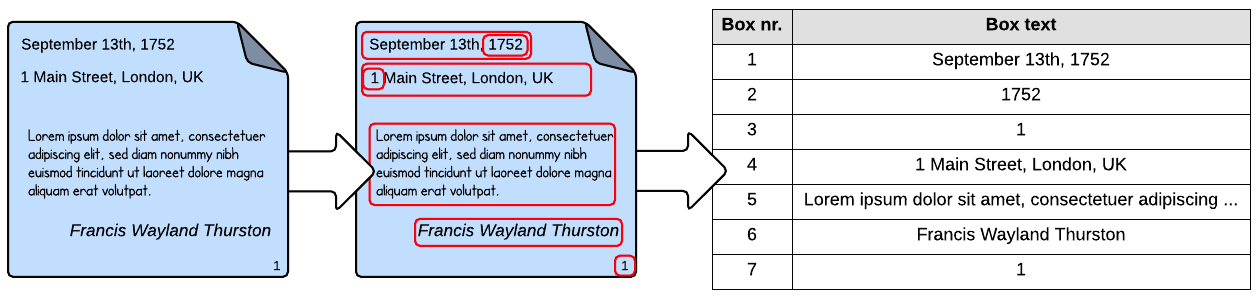
\includegraphics[width=0.9\textwidth]{FeatureExtraction1.png}
	    \end{center}
		\caption{document segmentation from Kaggle website \label{fig:FeatureExtraction1}}
	\end{figure}

		\subsubsection{label}
			Any sample is related to a label or more. This is the aim of the project: labelling the samples. As mentioned previously a label could for instance be 'date' or 'pageNumber'. The competition provide 33 labels. Those labels are not explicit, we don't know what they correspond to.

			To a given sample is associated a 33d label vector with values 0 or 1. As there can be many labels, the vector size is not necessary 1. \fref{fig:labelcsv} shows an example of a sample labelling.


		\subsubsection{files}
			The data provided for this competition by Tradeshift consist of 3 csv files. 

			\begin{itemize}
				\item train.csv: File containing the training data. It has mearly 1.7m lines of samples and 145 columns of features. Each cell has a either a real, a discrete, a boolean or a text value.
				\item trainLabels.csv: File containing label of data. It has a 3D array with mearly 1.7m lines of samples, 33 columns of labels and each cell is either 0 or 1.
				\item test.csv: File containing the testing data. It has mearly 0.4m lines of samples and 145 columns of features. Each cell has a either a real, a discrete, a boolean or a text value.
			\end{itemize}



	\subsection{evaluation}
		The work is evaluated by sending a csv file on the kaggle website. The csv file is then evaluated by the system.

		The csv file 'sampleSubmission.csv', is a 2 column csv file. On the first column is listed the sample number and a label and on the second column a prediction corresponding to this tupple {sample,label}.

		Once submited, the file receive a score through a scoring function. The fuction scoring used is the negative logarithm of the likelihood, averaged over $N_t$ test samples and $K$ labels.
		Mathematically, this function is defined as follow:

		\begin{equation} \label{eq1}
			\begin{split}
				LogLoss & = \frac{1}{N_t \cdot K} \sum_{idx=1}^{N_t \cdot K} LogLoss_{idx} \\
				&= \frac{1}{N_t \cdot K} \sum_{idx=1}^{N_t \cdot K} [-y_{idx} \log{\hat{y}_{idx}} - (1-y_{idx}) \log{1-\hat{y}_{idx}}] \\
		        &= \frac{1}{N_t \cdot K} \sum_{i=1}^{N_t} \sum_{j=1}^{K} [-y_{ij} \log{\hat{y}_{ij}} - (1-y_{ij}) \log{1-\hat{y}_{ij}}]
			\end{split}
		\end{equation}

		This function gives an extreme punishment for wrong confident predictions. 

		For instance, the logloss of one sample with one label predicting 0.001 intead of 1 (an extrealy confident wrong prediction) is $-\log(0.001) = 3 $ whereas the logloss of one sample with one label predicting 0.1 intead of 1 (a less confidently wrong prediction) is $\log(0.1) = 1$





	\subsection{Background}
		We aim at solving this problem learning a deep neuronal network.


		As proposed on the competition forum, the text input from the hash code, will be translated into a single binary entry. In other terms, a hash code looking like 'ASddeF54(fd=' will take a binary value '1001'. After formating those kind of inputs, the neural network will have a hash embedding layer with redundancy over the hash input layer. This layer will ensure an understanding of hash vocabulary code by the network. 

		As any features has a defined functions, we will try some different architectures of network. We will try to find the content, spacial, relational or parsing features to group them in for new embeding layers.

		Once those layers are defined, a last hidden layer will merge the results find an optimal answer for the stated problem.


